\chapter{Workspace Manager}
\label{ws_manager}
Workspace manager encapsulates all functionality of the parser library. It is the access point to all parsing capabilities, keeps the current state of all open files and resolves libraries needed by the analyzer. It also manages when files should be reparsed.


%******************** Parser library API *************************
\sectionSrc{Parser library API}
{parser\_library/include/protocol.h,parser\_library/include/range.h,parser\_library/include/workspace\_manager.h,parser\_library/src/workspace\_manager\_impl.h}
First of all, the workspace manager component is the only public interface of the parser library. The API design is based on LSP and DAP, most of the API is just LSP/DAP rewritten in C++. The API uses the observer pattern for DAP events and notifications originating in parser library (e.g. textDocument/publishDiagnostics).

The API can be divided into three categories:
\begin{itemize}
	\item Editor state and file content synchronization (\cref{text_sync_methods})
	\item Parsing results presentation 
	\item Macro tracer
\end{itemize}

\subsection{Editor state and file content synchronization}

\begin{table}
	\centering
	\begin{tabular}{ll}
		
		\toprule
		Method & Description \\ \midrule
		did\_open (file name, file content) & \multirow{3}{8cm}{Three methods that are called whenever the user opens a file, changes contents of an already opened file or closes a file in the editor.} \\
		did\_change (file name, changes)& \\
		did\_close (file name)& \\
		& \\
		\multirow{3}{5cm}{did\_change\_watched\_files(file paths)} &\multirow{3}{8cm}{Method, that is called when a file from a workspace has been changed outsize of the editor} \\
		& \\
		& \\
		& \\
		add\_workspace (ws name, ws path) & \multirow{2}{8cm}{Methods that are called when the user opens or closes a workspace in the editor} \\
		remove\_workspace (ws path) & \\ \bottomrule
	\end{tabular}
	
	\caption{List of all Editor state and text synchronization methods}
	\label{text_sync_methods}
\end{table}

All the methods from the first category are listed in \cref{text_sync_methods}. There are two types of files that need to be synchronised:
\begin{itemize}
	\item Files, that the user has opened in the editor. Those files are being edited by the user and their content may be different from the files actually saved in the filesystem.
	\item Files, that the parser library opens from the hard disk, because they are needed to parse opened files (e.g. a macro that is used by an opened file)
\end{itemize}

So the parser library is allowed to load arbitrary files from the disk, and use its contents until such file is opened in the editor. From that point on, the only source of truth for the contents of the file are the did\_change notifications. Once the file is closed in the editor, the parser library is again allowed to rely on its contents in the filesystem.



\subsection{Parsing results presentation}

\begin{table}
	\centering
	\begin{tabular}{ll}
		
		\toprule
		Method & Description \\ \midrule
		& \multirow{3}{8cm}{The method gets a position in an opened file. If there is a symbol, the method returns position of definition of that symbol} \\
		definition(file name, caret position) &  \\
		& \\
		& \\
		& \multirow{3}{8cm}{The method gets a position in an opened file. If there is a symbol, the method returns list of positions where the symbol is used}\\
		references(file name, caret position) & \\
		& \\
		& \\
		& \multirow{3}{8cm}{The method gets a position in an opened file where the user points with cursor. Returns list of strings to be shown in a tooltip window}\\
		hover(file name, mouse position)& \\
		& \\
		& \\
		& \multirow{3}{8cm}{The method gets a position in an opened file and how the completion box was triggered (i. e. with what key, automatically/manually). Returns list of strings suggested for completion at the position}\\
		completion(file name,& \\
		mouse position, trigger info)& \\
		& \\
		& \\ \bottomrule
	\end{tabular}
	
	\caption{List of all parse results methods}
	\label{parse_results}
\end{table}

All the methods from the second category are listed in \cref{parse_results}. They get position of caret or mouse cursor in a file and are expected to return information about the place in the code. For example, method \TT{hover} is called when the user points at some word in the code and waits for a short time. The method returns a string that the editor shows in the tooltip window at the position. Typically, the tooltip would show type of the variable and its value, if known.

Additionally, the parser library presents its results using the observer pattern. There are two interfaces: highligting and diagnostics consumer. Each of them has method \TT{consume} that gets updated information as parameter whenever there is an update. Any potential user of the library (e.g. the language server component) just has to implement the interfaces to process the results.

\subsection{Macro tracer}

The macro tracer part of the API is again just DAP rewritten in C++. There are methods that are called when the user clicks on buttons to control the macro tracer: launch the tracer, step in, step over, continue and stop. Moreover, there are methods that retrieve information about current state of traced code: stack of macro calls and information about compile time variables. See \cref{macro_tracer} for full description of macro tracer.

\section{Libraries configuration}
\label{libs_config}
The parser library approaches the dependency resolution in a way similar to the mainframe. On mainframe, you would have to define the locations of your dependencies in a JCL file \footnote{\url{https://www.ibm.com/support/knowledgecenter/zosbasics/com.ibm.zos.zjcl/zjclc_basicjclconcepts.htm}}. As the user may want to include tens of dependencies for multiple open codes, a source code management tool called Endevor\footnote{\url{https://en.wikipedia.org/wiki/Endevor}} groups these dependencies into so-called \emph{processor groups}. Then, the user only has to assign a processor group to the open code and the Endevor does the dependency resolution for him.

To provide similar experience with local files, the parser library simulates this behavior. If the user wants to include dependencies in his project, he has to define 2 configuration files inside his workspace: \emph{pgm\_conf.json} and \emph{proc\_grps.json}. The workspace component of the parser library then processes the configurations, retrieving their values upon initialization. Moreover, each time a save command is issued on any configuration file, the configuration values are reloaded via \TT{load\_config} method.

\subsection{Processor groups}

The proc\_grps configuration file contains a JSON array of possible processor groups, which consist of a name and an array of folder paths (may be relative to the root of the workspace). An example can be found in \cref{lst:proc_grps}.

Whenever \TT{load\_config} is called, the workspace retrieves these processor groups from the configuration file and creates libraries. The libraries provide information about paths to their dependency files. During the parsing, the workspace retrieves the library corresponding to the provided processor group name and uses it to search for a wanted macro or copy file. 

\subsection{Program configuration}

The pgm\_conf configuration file contains a JSON array of program names (or wildcards~\ref{section:wildcard}), matched to their processor groups. It serves as a list of the HLASM open code files and states the libraries (in form of processor groups) that contain the dependencies of each open code. An example can be found in \cref{lst:pgm_conf}.


From this configuration, the workspace simply remembers the processor group - open code mapping.


\begin{listing}[t]
	\begin{verbatim}
	{
	  "pgroups": [
	    {
	      "name":"GROUP1",
	      "libs": [
	        "ASMMAC/",
	        "C:/SYS.ASMMAC"
	      ]
	    },
	    {
	      "name":"GROUP2",
	      "libs": [
	        "G2MAC/",
	        "C:/SYS.ASMMAC"
	      ]
	    }
	  ]
	}
	\end{verbatim}
	\caption{A processor group configuration file}
	\label{lst:proc_grps}
\end{listing}

\begin{listing}[t]
	\begin{verbatim}
	{
	  "pgms": [
	    {
	      "program": "source_code",
	      "pgroup": "GROUP1"
	    },
	    {
	      "program": "second_file",
	      "pgroup": "GROUP2"
	    },
	  ]
	}
	\end{verbatim}
	\caption{A program configuration file}
	\label{lst:pgm_conf}
\end{listing}

\section{Architecture overview}
The architecture of the parser library is organized into the following components:

\begin{description}
	\item[Workspace manager API] The workspace manager provides API for handling various workspace management (e.g. add new workspace), LSP and DAP requests. It may hold multiple workspaces and calls 
	file manager to handle changes in the workspace files.
	\item[Workspace representation] The representation of workspace deals with the relations between its files (dependencies) upon parse request and propagates the parsing further into analyzer. It also retrieves data from the configuration files and it is used for resolving dependency searches by implementing parse library provider.
	\item[Processor group representation] \sectionFiles{.45\linewidth}{parser\_library/src/workspaces/processor\_group.h} 
	The representation of a processor group uses the API of libraries to search for their dependencies. Currently, we only support local libraries, which utilize the file manager for their file information retrieval.
	\item[File manager] \sectionFiles{.45\linewidth}{parser\_library/src/workspaces/file\_manager.h}
	The file manager is used by multiple components to handle file management and file searches. It also distinguishes and does conversions between regular files and processor files, which may be used for parsing.
	\item[Analyzer] The analyzer accepts a file along with the information needed for dependency resolution, syntactically and semantically processes it and fills the context tables. The component is further explained in~\cref{chap:analyzer}.
\end{description}

An overview of the architecture is visualised in~\cref{ws_mngr_arch}.

The technical details of each component are further explained in the following sections.

\afterpage{
\begin{landscape}
\begin{figure}
	\centering
	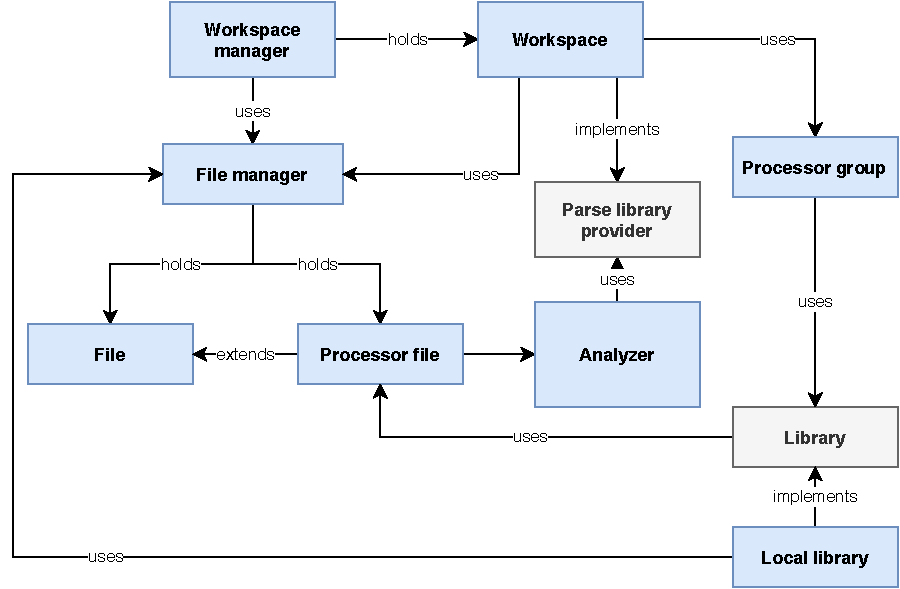
\includegraphics[width=16cm]{img/ws_mngr_arch}
	\caption{Architecture of workspace manager.}
	\label{ws_mngr_arch}
\end{figure}
\end{landscape}
}

%******************** Workspace *************************
\sectionSrc{Workspace representation}
{parser\_library/src/workspaces/workspace.h}

The representation of workspace is used by the workspace manager to handle various changes in the workspace. The workspace manager propagates LSP requests and notifications coming from the language server to the corresponding workspace and retrieves the results from it via the registered observers.

The workspace component uses the file manager for the file searches, retrieves the values from the configuration files and creates processor groups and is capable of resolving dependencies.

Due to the possibility to include files, the workspace maintains a list of dependants, which are  active dependencies of another workspace files. The list of dependants is needed, for example, in case the user changes contents of a macro that is used by multiple open code files, as all of them would have to be reparsed.

The core of the workspace is its \TT{parse\_file} method. As addition to the parsing part, it also ensures that the file to be parsed, its dependencies and dependants provide consistent results. The method works as follows:

\begin{enumerate}
	\item It checks whether the parsed file is a configuration file. If so, the workspace reloads the configuration values and reparses all dependants in the workspace.
	\item In case the parsed file is not a configuration file, it creates a list of all files to be parsed. This list consists of files depending on the parsed file and the parsed file itself.
	\item The method reparses the files in this list and creates new dependants, based on the dependencies reported from the parsing.
	\item It checks for the files that are no longer in use (former dependencies) and closes them.
\end{enumerate}

The workspace also ensures the correct closure of the file via \TT{didClose} method. It works as follows:

\begin{itemize}
	\item If the closed file is a dependency of some other file, it cannot be removed completely from the file manager, as it is still in use. The file manager is rather notified that the file was closed in the editor.
	\item If it is not a dependency, the method checks for its dependants and closes them. 
\end{itemize}                        

%******************** Files *************************
\sectionSrc[0.45\linewidth]{File Representation}
{parser\_library/src/workspaces/file.h,parser\_library/src/workspaces/file\_impl.h,parser\_library/src/workspaces/file.h,parser\_library/src/workspaces/processor.h,parser\_library/src/workspaces/processor\_file\_impl.h}

The file manager maintains all files across different workspaces. It distinguishes between regular, non-HLASM files and processable, HLASM files by using different representations.

The representation of a regular file (called \emph{file}) is capable of providing its file names, its contents and changing its state upon file-oriented LSP requests, i.e didChange, didClose and didOpen.

The representation of processor files is defined by \emph{processor\_file} class, which derives from both \emph{file} and \emph{processor} abstract classes. The \emph{processor} is an interface which is capable of actual processing (parsing). Its only implementation is processor file.

When the \TT{parse} method is invoked, the processor file initializes new analyzer, uses it for the parsing and rebuilds its dependencies list, closing the unwanted ones. When the parsing is finished, it keeps the instance of the analyzer and provides its parsing results when requested.


%******************** Libraries resolution *************************
\sectionSrc{Library path resolution}
{parser\_library/src/workspaces/parse\_lib\_provider.h,parser\_library/src/workspaces/library.h}

The libraries are resolved using a \emph{parse\_lib\_provider} interface. Whenever a component is to be used for dependency handling, it implements this interface and may be used by analyzer for this purpose.

The parse lib provider's \TT{parse\_library} method is passed the name of the library, the current context tables and the library data, which state what kind of processing is the analyzer using. When \TT{parse\_library} returns, library (i.e. a macro or COPY file) with the specified name is parsed and properly added to the context.

The workspace is the most important implementation of the \TT{parse\_library\_provider} interface. It provides libraries based on the processor groups configuration described in \cref{libs_config}.

%******************** Diagnosable *************************
\sectionSrc{Diagnostics}
{parser\_library/src/diagnosable.h,parser\_library/src/diagnosable\_impl.h,parser\_library/src/diagnostic.h}
A diagnostic is used to indicate a problem with source files, such as a compiler error or a warning. Some diagnostics are created in almost every component of the parser when it finds a problem with a source code. Diagnostics are also used in workspace to indicate problems with configuration files. After each parsing, we need to collect all the diagnostics from all the instances of all the components and pass them to the language server.

The components capable of collecting the diagnostics are organized in a tree where the root is the workspace manager. Starting from the root, each component collects the diagnostics of those children that are again capable of collecting or generating diagnostics.

To enforce this behavior, all of these components implement the \emph{diagnosable} interface. Its functionality is simple, it is used to add diagnostics, show his own and collect them from other diagnosable members. Each component that implements the interface is required to collect diagnostics from diagnosable objects it owns. In the result, one call of \TT{collect\_diags} from the root of the tree collects all diagnostics that were created since last such call.

The diagnosable hierarchy of workspace manager component is shown in \cref{diagnosable_hierarchy}.

\begin{figure}
	\centering
	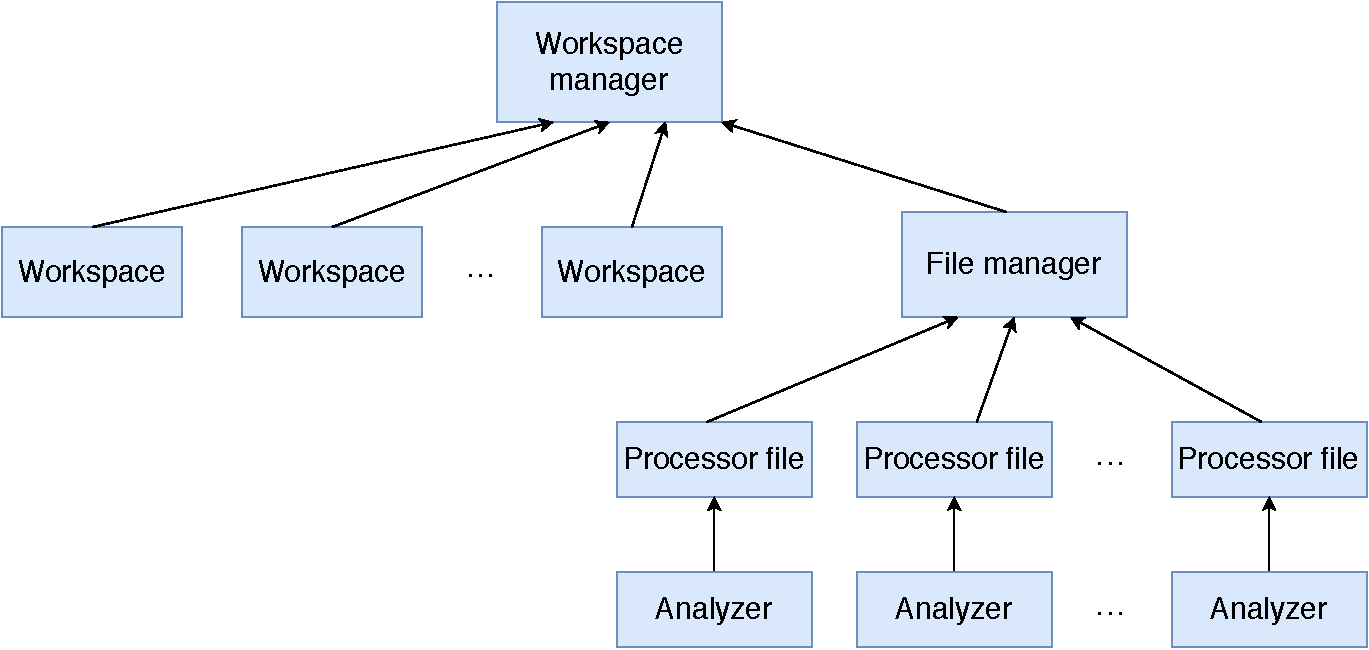
\includegraphics[width=\textwidth]{img/diagnosable_hierarchy}
	\caption{Hierarchy of diagnostics collection in the workspace manager component}
	\label{diagnosable_hierarchy}
\end{figure}